%===================================== CHAP 3 =================================

%\chapter{Method}
\chapter{Conceptual design}
%\chapter{Approach and methodology}

\section{Overall Approach}

%%forklare hva jeg prøver å gjøre på en generell måte. introdusere pipelinen
Wikipedia is a web page presenting articles for the user. This leads to high focus on the usability related to users searching and reading articles. Because of this one can say that their articles are stored as an atomic entity in their database. An articles has no internal structure, except for the markup used to present it. That means that a process is needed to identify and extract examples from Wikipedia articles. This 
project%%Hva burde jeg kalle dette?
looks into the pipeline technique for this process. As explained in section \ref{pipeline}, a pipeline consist of multiple independent processes loosely coupled.\\


%\section{Prerequisite knowledge}

\section{Pipeline}

%%Write something about the approach being for data mining. Where to different methods where explored. Focus on how it was done.

\subsection{Existing pipeline} \label{smila}

\begin{figure}[h]
\caption{An overall overview of the SMILA architecture}
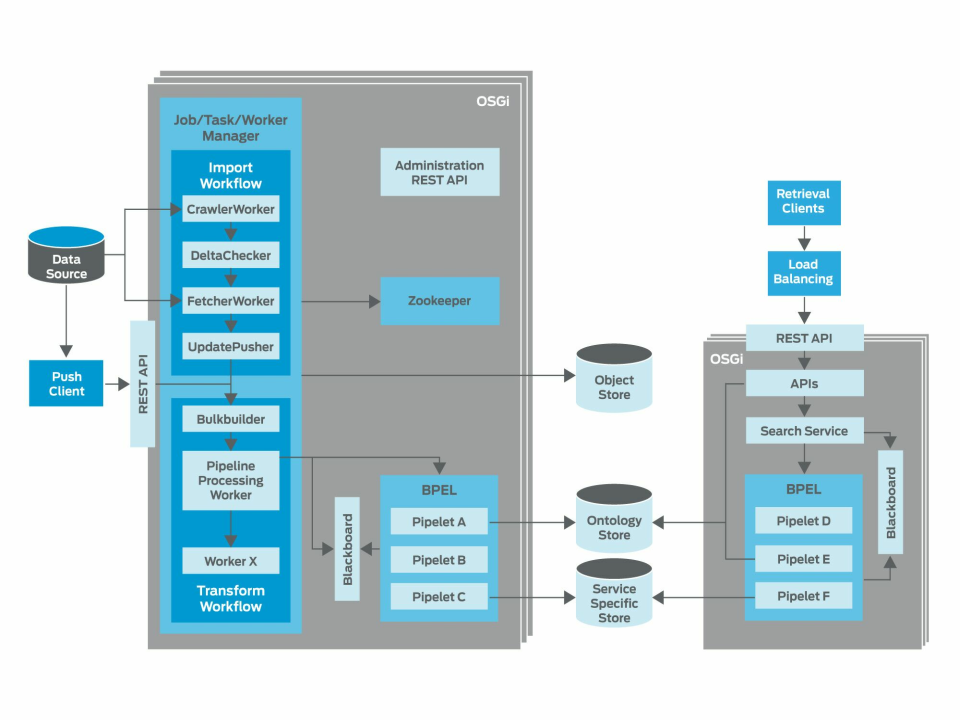
\includegraphics[width=\textwidth]{SMILA_Architecture}
\end{figure}

In the early stages of the project, an existing project called SMILA was explored. SMILA crawls the web to extract information and then stores the information in an index. It has a REST API to control the system and for searching the index. The SMILA architecture is also based on the pipeline architecture containing the following processes jobs, crawling, storage, indexing and querying. With SMILA being very complex, it gains asynchronicity as its biggest benefit from the pipeline architecture. The SMILA pipeline also allows custom made pipelets to be inserted into the pipeline. A pipelet is a sub process inside a pipeline. By creating pipelets, the behaviour of SMILA could be tailored into extracting the relevant information from Wikipedia.

By only writing pipelets and then make SMILA use them when crawling Wikipedia, the project could concentrate the effort on identifying and indexing the examples. Unfortunately SMILA is an old and complex system, and is rarely updated anymore. When problems running SMILA appeared, it was quite troublesome to understand why and fix the issue. This ironically lead to all the effort in the starting phase being used on making SMILA run properly, instead of looking into the characteristics of examples. 



\subsection{Creating pipeline from scratch} \label{custom-pipeline}

\begin{figure}[h]
\caption{A conceptual overview of the pipeline used to extract and index examples}
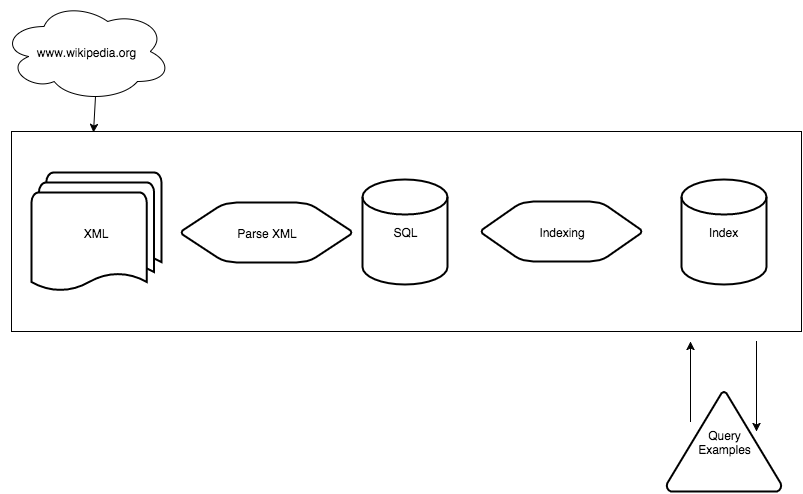
\includegraphics[width=\textwidth]{PipelineConcept}
\end{figure}

As described in section \ref{smila}, SMILA did not end up being a helpful tool for this project. Therefor other methods were considered, which mainly consisted of building the pipeline from scratch. Tailoring the different sub-processes for this project and organizing them in a pipeline, was decided to be the best course of action. The first issue to be settled regarded the format of the source data. SMILA was supposed to crawl www.wikipedia.org, but using a web-crawler is a very general method. Since this project were going to use wikipedia, it could be more specific. An XML-dump from a snapshot of wikipedia was considered the best solution. This dump contains all the articles of wikipedia in their newest version.

A parsing process was created in JavaScript running locally on a node.js server. This process iterates through every article and identifies sections with examples in them. It then parses that article into a JavaScript object with the relevant data. As it iterates over the articles, the process stores the data in a sql database with its new structure and relations. 

To allow an effortless fetching of data from the database a view was created. This view contains the fields that later in the pipeline will be used to build the index. Elasticsearch was chosen as tool for building the index. A simple java program fetches the view, containing the examples, from the database and builds an index. Elasticsearch serves a http API for querying of the index.

All the sub-processes in the pipeline are loosely coupled. This means that they are fully independent given the correct input. This also allows the pipeline to easily swap out sub-processes without affecting the rest of the system. The SMILA pipeline also delivered a high degree of parallelity. This is a property the current version of the pipeline created from scratch does not have. This is because functionality was prioritized above efficiency during development. 



\section{Database}

\begin{figure}[h] 
\caption{A simple overview of the database tables and their attributes}
\includegraphics[width=\textwidth]{db_diagram}
\label{fig:db_diagram}
\end{figure}

Section \ref{custom-pipeline} explains that the source data is fed into the pipeline as a snapshot of Wikipedia at a particular time. The size of the source data is an approximately 50 GB XML-document. Most of this data is not interesting in this project. Therefor the parser excludes most of it before it is structured in the SQL database. 

Figure \ref{fig:db_diagram} displays the tables of the database and the relations between them. If a relevant article is discovered, it is inserted into the \textit{pages} table. The article is found relevant because it contains one or more sections with an example. These sections are then stored in the database with their relation to the article. The categories of the article is also kept, because it will be helpful regarding searching among examples in the finished index.  

The database acts a temporary buffer for the data going into the index. This is helpful because it separates the parsing from the building of the index. This is preferred since the parsing is a very time consuming process, and having it structured in SQL with its meta data helps with showing how successful the parsing was. Most of the meta data is also irrelevant for the index, so only keeping it in the database is beneficial for complexity of the end result.



\section{Analysis of examples}
strucutre/characteristics of an example\\
what is good and bad example

\cleardoublepage